\subsection{Conectarse a una partida}

\begin{figure}[ht]
\centering
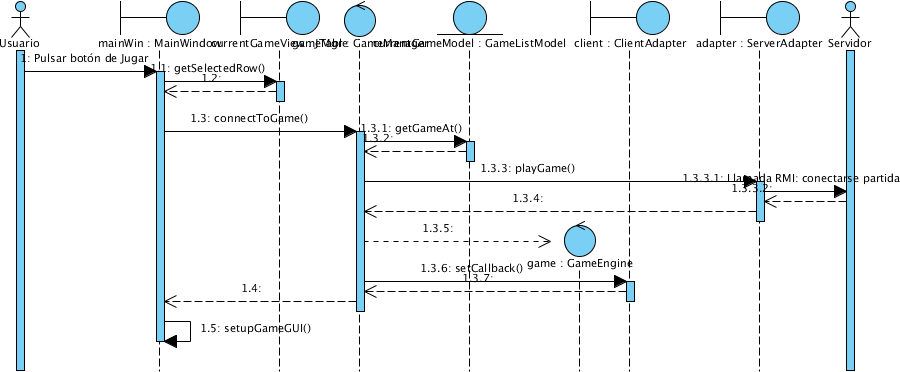
\includegraphics[scale=0.6]{img/ch03devel-playgame.png}
\caption{Diagrama de secuencia de ``Conectarse a una partida''}
\end{figure}

Si se selecciona una partida a la que el usuario ya se haya unido previamente,
podrá entonces ejecutar la acción de jugar en esa partida. Al igual que en el
caso anterior, la ventana principal obtendrá el índice de la partida a partir
de la vista.

El gestor de partidas realizará la petición al servidor de comenzar a jugar en
la partida seleccionada. Es entonces cuando el gestor de partidas creará un
objeto de tipo \texttt{GameEngine} a partir de los datos devueltos por el
servidor.

Esta clase está encargada de toda la lógica del juego, e implementa todos los
casos de uso relacionados con el módulo de juego. Dentro de ella se crean los
dos modelos de datos básicos en cada partida: \texttt{MapModel} y
\texttt{PlayerListModel}.

La clase \texttt{MapModel} almacena la información de los 42 territorios que
tiene una partida. Los datos de cada territorio son accesibles al completo a
través de la función \texttt{getTerritoryAt}. Sin embargo, si se accede a través
de la función \texttt{getValueAt} definida por el \textit{framework}, los datos
devueltos son filtrados de acuerdo a las reglas del juego. Esto es así porque
las vistas usarán esta última función, y de esta forma la vista no necesita
realizar ninguna lógica de control sobre los datos. La clase
\texttt{PlayerListModel} funciona de manera análoga con la lista de jugadores.

El motor del juego también debe responder a las peticiones que llegan del
servidor. Para ello se ha creado la interfaz \texttt{ClientCallback}, la cual
implementa. Una vez creado el objeto de tipo \texttt{GameEngine}, éste es
pasado al \texttt{ClientAdapter} para que redirija las peticiones que lleguen
del servidor.

Finalmente, cuando dominio ha terminado de preparar los datos, la ventana
principal carga la nueva interfaz de partida. Ésta está compuesta por tres
vistas: \texttt{MapView}, \texttt{PlayerView}, y \texttt{TerritoryInfoView}.

Todas estas vistas implementan la interfaz \texttt{TableModelListener}, a la
vez que se registran como observadores de los modelos correspondientes. La
vista \texttt{TerritoryInfoView} muestra información sobre el territorio
seleccionado en el mapa. Por ese motivo, esta clase también debe registrarse
como observador del modelo de selección de la clase \texttt{MapView}.
